\documentclass[11pt,a4paper]{article}
\usepackage[margin=1in,top=1.5in]{geometry}
\usepackage{graphicx}
\usepackage{hyperref}
\usepackage{fancyhdr}
\usepackage{sectsty}
\usepackage{titlesec}
\usepackage{enumitem}
\usepackage{parskip}
\usepackage{xcolor}
\usepackage{booktabs}
\usepackage{multicol}
\usepackage{float}

% Fix header height to prevent overlap
\setlength{\headheight}{45pt}
\setlength{\headsep}{20pt}

\definecolor{bracblue}{RGB}{0, 51, 102}
\definecolor{bracgold}{RGB}{204, 153, 0}

\hypersetup{
    colorlinks=true,
    linkcolor=bracblue,
    filecolor=bracblue,
    urlcolor=bracblue,
    citecolor=bracblue,
}

% Professional section formatting
\titleformat{\section}
  {\color{bracblue}\Large\bfseries}
  {\thesection}{1em}{}
  [\titlerule]

\titleformat{\subsection}
  {\color{bracblue}\large\bfseries}
  {\thesubsection}{1em}{}

\sectionfont{\color{bracblue}}
\subsectionfont{\color{bracblue}}

\pagestyle{fancy}
\fancyhf{}
\rhead{
\includegraphics[width=1.5cm]{Images/Logo/brac-university-logo.png}}
\lhead{\footnotesize Qiskit Fall Fest 2025 Workshop Report}
\rfoot{\footnotesize Page \thepage}

\title{
    \vspace{-1cm}
    \begin{center}
        
\includegraphics[width=0.2\textwidth]{Images/Logo/brac-university-logo.png}\\[0.5cm]
        {\Huge\textbf{Qiskit Fall Fest 2025}} \\[0.3cm]
        {\Large Celebrating a Century of Quantum Computing} \\[0.3cm]
        {\large Comprehensive Workshop Operations Report}
    \end{center}
    \vspace{-0.5cm}
}
\author{
    \normalsize BRAC University Quantum Computing Initiative
}
\date{}

\begin{document}

\maketitle

\thispagestyle{empty}

\newpage

\tableofcontents

\newpage

\section{Executive Summary}

This comprehensive report details the operational framework for the Qiskit Fall Fest 2025 workshop, hosted by BRAC University's student-led team in collaboration with IBM Quantum. The event, themed ``Celebrating a Century of Quantum Computing," is scheduled from October 14 to October 18, 2025. It adopts a hybrid format, combining in-person and online sessions to engage 50--100 STEM students in quantum computing fundamentals, hands-on Qiskit training, and a mini-hackathon.

The workshop aims to build foundational skills in quantum computing, foster innovation through collaborative projects, and identify 4--6 top performers for participation in MIT iQuHACK 2026. Key components include expert talks, interactive labs, and a competitive hackathon utilizing IBM's official hackathon package.

Roles have been assigned to ensure seamless execution: Abdullah Al Omar Galib as Representator, Ziya Mohammad Sayef Ullah as Club Logistics Coordinator, TISAM SAJRAN as Logistics Coordinator, MD. Foysal as Event Manager, and Md. Rejoan Mehedi as Marketing Lead.

Potential speakers include Dr. Tibra Ali for the opening talk and Mr. Sowmitra Das for the closing session, leveraging their expertise in theoretical physics and quantum information theory.

This report outlines the event structure, schedule, participant requirements, team roles, and evaluation criteria to guarantee a professional, impactful experience.

\section{Event Overview}

The Qiskit Fall Fest 2025 is a 4-day workshop designed to commemorate the International Year of Quantum Science and Technology. It targets undergraduate and graduate students in physics, computer science, engineering, and related fields, as well as early-career researchers and industry professionals curious about quantum computing.

\textbf{Dates:} October 14--18, 2025 (with October 17 as a dedicated project day).  
\textbf{Duration:} 2 hours per session (5:00 PM--7:00 PM BST).  
\textbf{Format:} Hybrid -- in-person at BRAC University's theatre room for Days 1, 2, and 4; online via Zoom for Day 3 and hackathon support.  
\textbf{Participants:} 50--100 students from Physics, EEE, computer science, and robotics clubs.  
\textbf{Objectives:} 
\begin{itemize}
    \item Educate on quantum basics (superposition, entanglement).
    \item Teach quantum gates, circuits, and Qiskit framework.
    \item Facilitate hands-on coding and project collaboration.
    \item Explore quantum computing history and future.
    \item Select top performers for MIT iQuHACK 2026 via mini-hackathon.
\end{itemize}

Participants require basic Python knowledge, familiarity with linear algebra, and a personal laptop. No prior quantum experience is needed.

\section{Workshop Schedule}

The schedule is structured around daily themes, blending lectures, labs, and hackathon activities. All sessions occur from 5:00 PM--7:00 PM BST.

\subsection{Day 1: Kick-off and Inspiration (Tuesday, October 14 -- In-Person)}
\begin{itemize}
    \item 5:00 PM--5:15 PM: Welcome and overview.
    \item 5:15 PM--6:15 PM: Opening talk by Dr. Tibra Ali on ``Celebrating a Century of Quantum."
    \item 6:15 PM--7:00 PM: Hackathon kick-off -- theme announcement, IBM platform demo, rules, judging criteria, team formation via Discord.
\end{itemize}

\subsection{Day 2: Quantum Basics \& Qiskit (Wednesday, October 15 -- In-Person)}
\begin{itemize}
    \item 5:00 PM--6:00 PM: Talk on quantum information (qubits, superposition, entanglement).
    \item 6:00 PM--7:00 PM: Lab -- Qiskit setup, creating first qubits.
\end{itemize}

\subsection{Day 3: Building Quantum Circuits (Thursday, October 16 -- Online)}
\begin{itemize}
    \item 5:00 PM--6:00 PM: Talk \& Lab -- Quantum gates, complex circuits, simulator runs.
    \item 6:00 PM--7:00 PM: Q\&A and hackathon support.
\end{itemize}

\subsection{Day Off (Friday, October 17)}
No sessions; dedicated to hackathon project work.

\subsection{Day 4: Final Talks \& Hackathon Showcase (Saturday, October 18 -- In-Person)}
\begin{itemize}
    \item 5:00 PM: Hackathon submissions due.
    \item 5:00 PM--6:00 PM: Closing talk by Mr. Sowmitra Das on quantum computation advancements.
    \item 6:00 PM--6:45 PM: Hackathon showcase -- top 3 presentations, winner announcements.
    \item 6:45 PM--7:00 PM: Certificates and closing remarks.
\end{itemize}

\section{Roles and Responsibilities}

To ensure efficient operations, the following team members have been assigned key roles based on their expertise and experience:

\begin{description}[style=nextline,leftmargin=2em]
    \item[\textbf{Representative: Abdullah Al Omar Galib}] 
    Serves as the primary liaison with IBM Quantum and external stakeholders. Responsibilities include representing the event at collaborations, overseeing quantum education content, and mentoring participants. 
    
    \textbf{CV:} \href{https://ahkatlio.github.io/Ahkatlio_CV/cv.pdf}{View Profile}
    
    \item[\textbf{Club Logistics Coordinator: Ziya Mohammad Sayef Ullah}] 
    Manages club-level logistics, including venue setup, equipment procurement, and inter-club coordination. Leverages experience in robotics and event management. 
    
    \textbf{CV:} \href{https://github.com/ahkatlio/Fall-Fest/blob/master/CV/Sayefs\%20CV\%20.pdf}{View Profile}
    
    \item[\textbf{Logistics Coordinator: TISAM SAJRAN}] 
    Handles day-to-day logistics such as participant registration, hybrid setup (Zoom/Discord), and resource distribution. Draws on skills in robotics, quantum computing, and team leadership. 
    
    \textbf{CV:} \href{https://github.com/ahkatlio/Fall-Fest/blob/master/CV/TISAM\%20SAJRAN.pdf}{View Profile}
    
    \item[\textbf{Event Manager: MD. Foysal}] 
    Oversees overall event execution, timeline adherence, and on-site management. Utilizes expertise in project management, robotics, and leadership. 
    
    \textbf{CV:} \href{https://github.com/ahkatlio/Fall-Fest/blob/master/CV/MD.\%20Foysal's\%20Resume.pdf}{View Profile}
    
    \item[\textbf{Marketing Lead: Md. Rejoan Mehedi}] 
    Leads promotion efforts, participant outreach, and branding. Applies skills in public relations, event volunteering, and communication. 
    
    \textbf{CV:} \href{https://github.com/ahkatlio/Fall-Fest/blob/master/CV/Curriculum\%20Vitae\%20of\%20Md.\%20\%20Rejoan\%20\%20Mehedi.pdf}{View Profile}
\end{description}

\section{Potential Speakers}

Expert talks are integral to inspiring participants. The following renowned professionals have been identified for the opening and closing sessions:

\subsection{Opening Talk: Dr. Tibra Ali}

\begin{figure}[H]
    \centering
    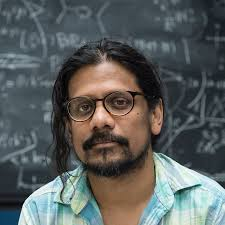
\includegraphics[width=4cm]{Images/People/Tibra_Ali.png}
    \caption{Dr. Tibra Ali}
\end{figure}

\noindent Dr. Tibra Ali is a theoretical physicist specializing in string theory, quantum field theory, and holographic duality. With over a decade of teaching experience at institutions like the Perimeter Institute for Theoretical Physics, Canada, he is passionate about elevating physics and mathematics education in Bangladesh. His talk will set the tone for the workshop's theme. 

\textbf{Profile:} \href{https://scholar.google.com/citations?user=mnfuAGsAAAAJ&hl=en}{Google Scholar Profile}

\subsection{Closing Talk: Mr. Sowmitra Das}

\begin{figure}[H]
    \centering
    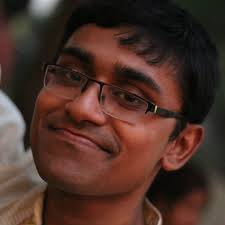
\includegraphics[width=4cm]{Images/People/sowmitra das.png}
    \caption{Mr. Sowmitra Das}
\end{figure}

\noindent Mr. Sowmitra Das, a lecturer at BRAC University's Department of Computer Science and Engineering, has a diverse background in Physics, EEE, theoretical physics, applied mathematics, and quantum computation. He co-taught Bangladesh's first academic quantum computing course and focuses on quantum information theory. His closing remarks will highlight future directions in the field.

\textbf{Profile:} \href{https://www.researchgate.net/profile/Sowmitra-Das}{ResearchGate Profile}

\section{Mini-Hackathon Details}

The mini-hackathon utilizes IBM's official package, providing participants with comprehensive tutorials and access to quantum systems. Project evaluation criteria include:

\begin{enumerate}[leftmargin=*]
    \item \textbf{Creative Ideas:} Originality and innovation in approach
    \item \textbf{Good Code:} Correct implementation of quantum concepts and algorithms
    \item \textbf{Impact:} Real-world applicability and potential societal benefit
    \item \textbf{Clear Pitch:} Quality of presentation and communication skills
\end{enumerate}

\textbf{Prizes and Recognition:}
\begin{itemize}[leftmargin=*]
    \item Digital certificates for all participants
    \item BRAC University branded merchandise for top performers
    \item Technology gadgets for hackathon winners
    \item Selection of top 4--6 participants for MIT iQuHACK 2026
\end{itemize}

\section{Conclusion}

The Qiskit Fall Fest 2025 represents a significant milestone in quantum computing education at BRAC University. Through meticulous planning, expert coordination, and clearly defined roles, this workshop is designed to deliver a structured and engaging experience that will advance quantum literacy among participating students.

The hybrid format ensures maximum accessibility while maintaining high-quality educational standards. With distinguished speakers, hands-on laboratory sessions, and a competitive hackathon component, participants will gain both theoretical knowledge and practical skills in quantum computing.

This initiative positions BRAC University as a leader in quantum education in Bangladesh and establishes a foundation for future quantum computing research and education programs. The event promises to inspire the next generation of quantum innovators and contribute to the global quantum computing community.

\vspace{1cm}

\begin{center}
\rule{0.8\textwidth}{0.4pt}\\[0.3cm]
BRAC University Quantum Computing Initiative \\
\textit{Preparing Tomorrow's Quantum Leaders}
\end{center}

\end{document}